% Graded Status in Ordinary Mathematics:
% Structure Preservation, Topology, and Analysis
%
% References to Lean formalization: lean/Cred/Approx, lean/Cred/Topology,
% lean/Cred/Math

\documentclass[11pt,a4paper]{article}

\usepackage{amsmath,amssymb,amsthm}
\usepackage{mathtools}
\usepackage{enumitem}
\usepackage{booktabs}
\usepackage{caption}
\usepackage{hyperref}
\hypersetup{
    colorlinks=true,
    linkcolor=blue,
    citecolor=blue,
    urlcolor=blue,
    pdfauthor={Christopher Albert},
    pdftitle={Graded Status in Ordinary Mathematics: Structure Preservation, Topology, and Analysis}
}
\usepackage{cleveref}
\usepackage[margin=1in]{geometry}
\emergencystretch=3em
\usepackage{tikz}
\usetikzlibrary{arrows.meta,positioning,shapes}
\usepackage{graphicx}
\usepackage{pgfplots}
\pgfplotsset{compat=1.18}

% Theorem environments
\newtheorem{theorem}{Theorem}[section]
\newtheorem{lemma}[theorem]{Lemma}
\newtheorem{proposition}[theorem]{Proposition}
\newtheorem{corollary}[theorem]{Corollary}
\newtheorem{definition}[theorem]{Definition}
\newtheorem{example}[theorem]{Example}
\newtheorem{remark}[theorem]{Remark}

% Custom commands
\newcommand{\cred}{\mathsf{cred}}
\newcommand{\negc}{\mathord{\sim}}
\newcommand{\conjc}{\otimes}
\newcommand{\disjc}{\sqcup}
\newcommand{\condc}[2]{({#1} \mid {#2})}
\newcommand{\Cond}{\mathsf{Cond}}
\newcommand{\Real}{\mathbb{R}}
\newcommand{\Nat}{\mathbb{N}}

\title{Graded Status in Ordinary Mathematics:\\
Structure Preservation, Topology, and Analysis}

\author{Christopher Albert\\
\small Institute for Theoretical and Computational Physics\\
\small Graz University of Technology}
\date{June 2026}

\begin{document}

\maketitle

\begin{abstract}
We attach a uniform status scale to ordinary mathematics: a
\emph{structure} on a carrier $X$ is a score $P : X \to [0,1]$, exact
preservation is the class $P\,x = 1$, and a threshold $t$ relaxes
exactness to $t \le P\,x$.
Classical on/off properties embed as $0/1$ scores; structure-preserving
maps form a monoid under composition; and a single clipped-linear
recipe $\mathrm{score}_\varepsilon(r) = \max(0, \min(1, 1 - r/\varepsilon))$
manufactures every graded degree from a residual and a scale.
We instantiate the scale three times.
On numerical structure preservation: positivity, the probability simplex,
monotonicity, maximum principles, the unit circle, first integrals,
$2 \times 2$ symplecticity ($A^{\top} J A = J \iff \det A = 1$),
finite-volume mass conservation by telescoping fluxes, positivity under
the bound $c\,\Delta t \le 1$, Lie-group steps, divergence-free
constraints, the cochain identity $d_1 \circ d_0 = 0$, energy balance,
and persistence; each structure carries a preserving scheme and a
value-accurate scheme that destroys it.
On topology: clopenness is the consistent conjunction
$\mathrm{Open}(s) \wedge \mathrm{Open}(s^{c})$, never $P \wedge \neg P$;
graded openness degrees collapse to $\{0,1\}$ on crisp sets; threshold
cuts of a graded set form an antitone family of crisp sets; and
clopen verdicts become threshold-relative.
On analysis: arithmetic laws sit at certainty, graded limits coincide
exactly with the standard limit, and a robustness audit separates % slop-ok: formal audit term
robust, branch-dependent, and inadmissible claims. % slop-ok: formal audit verdict
The underlying preservation theory, topology, and analysis are
classical; the contribution is the uniform status vocabulary.
All results are machine-checked in Lean~4 with Mathlib.
\end{abstract}

%=============================================================================
\section{Introduction}
\label{sec:intro}
%=============================================================================

Take one explicit Euler step of scalar decay.
Start at $x = \tfrac{1}{2}$, take step $h = 1$: the update
$x \mapsto x - h$ returns $-\tfrac{1}{2}$.
The input was a density, a probability, a concentration; the output is
negative.
The local value error is of the same order as the step, but that number
misses the failure: the scheme has left the set of objects it computes
on.
A negative density is not an inaccurate density.

The credence framework records this as a change of \emph{status}.
Nonnegativity is a score $P : \Real \to [0,1]$ with $P\,x = 1$ on
$x \ge 0$ and $P\,x = 0$ elsewhere; the bad step carries a point of
score $1$ to a point of score $0$
(machine-checked, \texttt{explicitEuler\_counterexample}).
Value accuracy and structural admissibility are different columns of
the ledger, and this paper keeps them apart on one scale.

\textbf{Honest scope.}
The preservation mathematics is not ours.
Symplectic and variational integrators win long-time behavior by
preserving the symplectic form, not by shrinking local
error~\cite{hairer2006,marsden2001};
Lie-group methods keep the flow on the
manifold~\cite{iserles2000};
strong-stability-preserving schemes keep densities nonnegative under
explicit steps~\cite{gottlieb2001};
finite element exterior calculus reproduces $d \circ d = 0$
discretely~\cite{arnold2006};
finite-volume schemes conserve mass by telescoping
fluxes~\cite{leveque2002};
persistent homology summarizes a filtration by a stable
diagram~\cite{edelsbrunner2010}.
The topology and analysis we touch are Mathlib's.
What this paper adds is one machine-checked status scale on which all
of these guarantees, and their failures, are stated and compared.
Throughout we separate three claim statuses:
\emph{established} (the cited literature and Mathlib, reused without
modification),
\emph{checked} (every theorem carrying a Lean name, verified by
\texttt{lake build} with no \texttt{sorry}), and
\emph{positioning} (the claim that one scale is the right common
denominator, which is argued, not proved).

\textbf{Main content.}
Section~\ref{sec:scale} defines the scale: structure degree, exact and
threshold preservation, the crisp embedding, the composition monoid
(Theorem~\ref{thm:monoid}), and the clipped-linear score
(Theorem~\ref{thm:score}).
Section~\ref{sec:numerics} instantiates it on six elementary structures,
each with a preserving scheme and a counterexample scheme
(Theorems~\ref{thm:positivity}--\ref{thm:firstintegral}).
Section~\ref{sec:geometric} covers geometric and conservative
integrators: the determinant characterization of $2 \times 2$
symplecticity (Theorem~\ref{thm:sympdet}), telescoping mass
conservation (Theorem~\ref{thm:fv}), the positivity bound
$c\,\Delta t \le 1$ (Theorem~\ref{thm:ssp}), Lie-group and constraint
preservation, the cochain identity (Theorem~\ref{thm:dd}), energy
balance, and persistence, then compares everything in
Table~\ref{tab:comparison}.
Section~\ref{sec:topology} grades topology: clopenness as a consistent
conjunction (Theorem~\ref{thm:clopen}), crisp recovery of classical
open sets (Theorem~\ref{thm:crisp-topology}), openness degrees, and
threshold cuts (Theorem~\ref{thm:cuts}).
Section~\ref{sec:analysis} treats arithmetic and analysis: laws at
certainty, the coincidence of graded and standard limits
(Theorem~\ref{thm:tlimit}), and a robustness audit
(Theorem~\ref{thm:audit}).
All theorems are machine-checked in Lean~4 with Mathlib
(Appendix~\ref{app:lean}).

%=============================================================================
\section{The Status Scale}
\label{sec:scale}
%=============================================================================

\subsection{Structure degree and preservation classes}

\begin{definition}[Structure, structure degree]
\label{def:structure}
Let $X$ be a set.
A \emph{structure} on $X$ is a function $P : X \to [0,1]$.
The \emph{structure degree} of $x \in X$ is
\[
  \deg_P(x) \;=\; P\,x .
\]
(Machine-checked, \texttt{StructureDegree}.)
\end{definition}

\begin{definition}[Preservation classes]
\label{def:classes}
For a structure $P$ on $X$, $x \in X$, and a threshold $t \in [0,1]$:
\begin{enumerate}[label=(\alph*),nosep]
\item $x$ \emph{exactly preserves} $P$ when $\deg_P(x) = 1$
  (machine-checked, \texttt{ExactPreserves});
\item $x$ \emph{preserves $P$ at threshold $t$} when
  $t \le \deg_P(x)$
  (machine-checked, \texttt{PreservesAt});
\item $x$ is \emph{admissible at $t$} when it preserves $P$ at $t$
  (machine-checked, \texttt{AdmissibleApprox}).
\end{enumerate}
\end{definition}

\begin{definition}[Crisp score]
\label{def:crisp}
For a decidable predicate $Q$ on $X$, the \emph{crisp score} is
\[
  \mathrm{crisp}_Q(x) \;=\;
  \begin{cases}
    1 & \text{if } Q\,x, \\
    0 & \text{otherwise.}
  \end{cases}
\]
(Machine-checked, \texttt{crispScore}.)
\end{definition}

\begin{definition}[Preserving map]
\label{def:preserves}
A self-map $\Phi : X \to X$ \emph{preserves} the structure $P$ when it
keeps the exact-preservation class:
$P\,x = 1$ implies $P\,(\Phi\,x) = 1$ for every $x$
(machine-checked, \texttt{Preserves}).
\end{definition}

\begin{proposition}[Endpoints and monotonicity of the threshold scale]
\label{thm:endpoints}
For every structure $P$, point $x$, and thresholds $s \le t$:
\begin{enumerate}[label=\textup{(\alph*)},nosep]
\item $x$ preserves $P$ at threshold $0$;
\item $x$ exactly preserves $P$ iff it preserves $P$ at threshold $1$;
\item exact preservation implies preservation at every threshold;
\item preservation at $t$ implies preservation at $s$;
\item $x$ exactly preserves $\mathrm{crisp}_Q$ iff $Q\,x$.
\end{enumerate}
\end{proposition}
\begin{proof}
(a) $0 \le P\,x$.
(b) $t \le P\,x \le 1$ with $t = 1$ forces $P\,x = 1$; the converse is
reflexivity.
(c) $t \le 1 = P\,x$.
(d) $s \le t \le P\,x$.
(e) The indicator equals $1$ exactly on $Q$, since $0 \neq 1$.
(Machine-checked, \texttt{preservesAt\_zero},
\texttt{exactPreserves\_iff\_preservesAt\_one},
\texttt{preservesAt\_of\_exactPreserves},
\texttt{preservesAt\_mono},
\texttt{exactPreserves\_crispScore}.)
\end{proof}

\Cref{fig:scale} shows the scale: a structure degree in $[0,1]$, the
threshold $t$ separating inadmissible from admissible, and the exact
class at the top.
The three regions are the numerical mirror of the status taxonomy of
the credence framework: certainty at $1$, threshold designation on
$[t,1)$, inadmissibility below $t$.

\begin{figure}[ht]
\centering
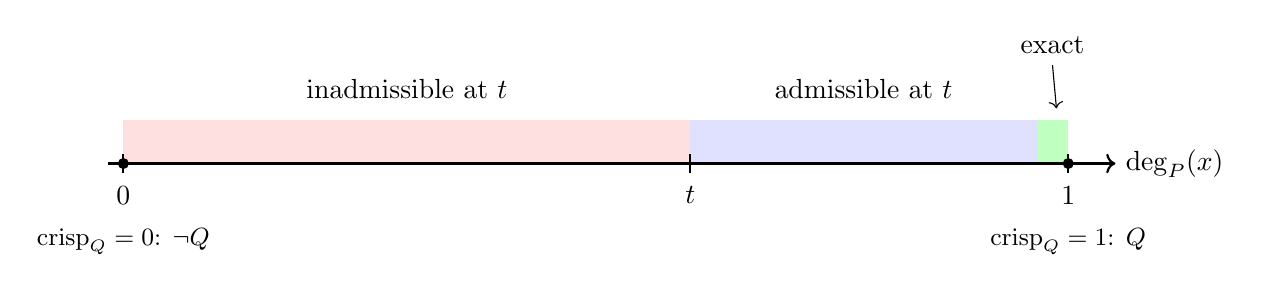
\begin{tikzpicture}[scale=1.0]
  % shaded regions
  \fill[red!12]    (0,0)   rectangle (7.2,0.55);
  \fill[blue!12]   (7.2,0) rectangle (11.6,0.55);
  \fill[green!25]  (11.6,0) rectangle (12,0.55);
  % axis
  \draw[->,thick] (-0.2,0) -- (12.6,0) node[right] {$\deg_P(x)$};
  % ticks
  \foreach \x/\l in {0/{$0$}, 7.2/{$t$}, 12/{$1$}}
    \draw[thick] (\x,-0.12) -- (\x,0.12) node[below=8pt] {\l};
  % labels
  \node at (3.6,0.95)  {inadmissible at $t$};
  \node at (9.4,0.95)  {admissible at $t$};
  \node at (11.8,1.5) {exact};
  \draw[->] (11.8,1.25) -- (11.85,0.7);
  % crisp embedding markers
  \fill (0,0) circle (2pt);
  \fill (12,0) circle (2pt);
  \node[below=20pt] at (0,0)  {\small $\mathrm{crisp}_Q = 0$: $\neg Q$};
  \node[below=20pt] at (12,0) {\small $\mathrm{crisp}_Q = 1$: $Q$};
\end{tikzpicture}
\caption{The structure-degree scale.
A threshold $t$ splits $[0,1]$ into an inadmissible region
$[0,t)$ and an admissible region $[t,1]$; the exact-preservation class
is the single point $1$.
A classical predicate $Q$ embeds at the two endpoints via
$\mathrm{crisp}_Q$ (\cref{def:crisp}).}
\label{fig:scale}
\end{figure}

\begin{theorem}[Preserving maps form a monoid]
\label{thm:monoid}
For every structure $P$ on $X$, the identity preserves $P$, and if
$\Phi$ and $\Psi$ preserve $P$, so does $\Psi \circ \Phi$
(machine-checked, \texttt{preserves\_id}, \texttt{preserves\_comp}).
\end{theorem}
\begin{proof}
$P\,x = 1$ gives $P\,x = 1$ for the identity.
For the composite: $P\,x = 1$ implies $P\,(\Phi\,x) = 1$ implies
$P\,(\Psi(\Phi\,x)) = 1$.
\end{proof}

A multistage method built from admissible substeps is therefore
admissible with no further proof obligation.

\subsection{The clipped-linear score}
\label{sec:score}

Every graded (non-crisp) degree in this paper comes from one recipe:
a nonnegative residual $r$ over a documented scale $\varepsilon$,
clipped linearly into $[0,1]$.

\begin{definition}[Clipped-linear score]
\label{def:score}
For $\varepsilon > 0$ and $r \in \Real$,
\[
  \mathrm{score}_\varepsilon(r)
  \;=\; \max\bigl(0,\; \min\bigl(1,\; 1 - r/\varepsilon\bigr)\bigr).
\]
(Machine-checked, \texttt{scoreEps}; packaged as a credence by
\texttt{scoreEpsCredence}.)
\end{definition}

\begin{theorem}[Properties of the clipped-linear score]
\label{thm:score}
Let $\varepsilon > 0$ and $r, r_1, r_2 \ge 0$.
Then:
\begin{enumerate}[label=\textup{(\roman*)},nosep]
\item $0 \le \mathrm{score}_\varepsilon(r) \le 1$
  (machine-checked, \texttt{scoreEps\_nonneg},
  \texttt{scoreEps\_le\_one});
\item $\mathrm{score}_\varepsilon(r) = 1$ iff $r = 0$
  (machine-checked, \texttt{scoreEps\_eq\_one\_iff});
\item if $\varepsilon \le r$ then $\mathrm{score}_\varepsilon(r) = 0$
  (machine-checked, \texttt{scoreEps\_zero\_of\_ge});
\item if $r_1 \le r_2$ then
  $\mathrm{score}_\varepsilon(r_2) \le \mathrm{score}_\varepsilon(r_1)$
  (machine-checked, \texttt{scoreEps\_antitone}).
\end{enumerate}
\end{theorem}
\begin{proof}
(i) The outer $\max$ with $0$ bounds below; the inner $\min$ with $1$
bounds above.
(ii) For $r = 0$: $1 - 0/\varepsilon = 1$, so the clip returns $1$.
Conversely $\mathrm{score}_\varepsilon(r) = 1$ forces
$\min(1, 1 - r/\varepsilon) = 1$, hence $1 \le 1 - r/\varepsilon$,
hence $r/\varepsilon \le 0$; with $r \ge 0$ and $\varepsilon > 0$ this
gives $r = 0$.
(iii) $\varepsilon \le r$ gives $1 - r/\varepsilon \le 0$, so the inner
$\min$ equals $1 - r/\varepsilon \le 0$ and the outer $\max$ returns
$0$.
(iv) Division by $\varepsilon > 0$ preserves order, so
$1 - r_2/\varepsilon \le 1 - r_1/\varepsilon$; $\min$ and $\max$ with
constants are monotone.
\end{proof}

\begin{figure}[ht]
\centering
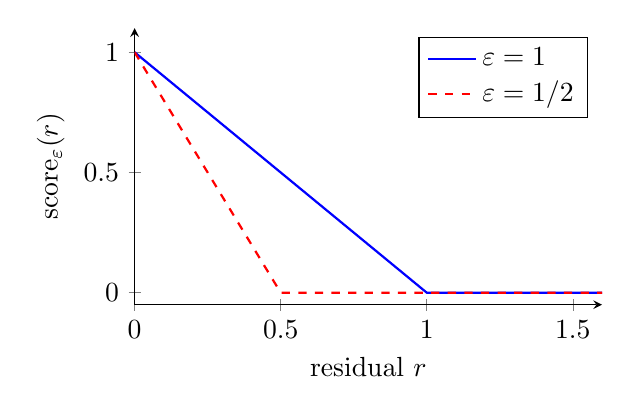
\begin{tikzpicture}
\begin{axis}[
    width=0.62\textwidth, height=0.42\textwidth,
    xlabel={residual $r$},
    ylabel={$\mathrm{score}_\varepsilon(r)$},
    xmin=0, xmax=1.6, ymin=-0.05, ymax=1.1,
    xtick={0,0.5,1,1.5},
    ytick={0,0.5,1},
    legend pos=north east,
    legend cell align=left,
    axis lines=left,
]
\addplot[blue, thick] coordinates {(0,1) (1,0) (1.6,0)};
\addlegendentry{$\varepsilon = 1$}
\addplot[red, thick, dashed] coordinates {(0,1) (0.5,0) (1.6,0)};
\addlegendentry{$\varepsilon = 1/2$}
\end{axis}
\end{tikzpicture}
\caption{The clipped-linear score of \cref{def:score} for two scales.
The score ramps from $1$ at zero residual down to $0$ at
$r = \varepsilon$ and stays there (Theorem~\ref{thm:score}(ii),(iii));
it is antitone in the residual (Theorem~\ref{thm:score}(iv)).}
\label{fig:score}
\end{figure}

The residual and scale for each structure are documented in the Lean
development; no status number in Table~\ref{tab:comparison} is chosen
by hand.

%=============================================================================
\section{Six Structures, Six Paired Schemes}
\label{sec:numerics}
%=============================================================================

Each subsection fixes one structure $P$, one preserving scheme, and one
value-plausible scheme that destroys the structure.
The positive theorem carries the admissibility hypothesis (a parameter
or step-size range); the counterexample exhibits a point of the exact
class whose image leaves it.

\subsection{Positivity}

\begin{definition}[Nonnegativity structure, paired schemes]
\label{def:positivity}
On $X = \Real$, let $P_{\ge 0} = \mathrm{crisp}_{\{x \,:\, 0 \le x\}}$
(machine-checked, \texttt{nonnegScore}).
For $a \ge 0$ define the implicit update and, for $h > 0$, the explicit
Euler subtraction:
\[
  \Phi_a(x) = \frac{x}{1 + a x},
  \qquad
  \Psi_h(x) = x - h .
\]
\end{definition}

\begin{theorem}[Positivity preservation]
\label{thm:positivity}
For every $a \ge 0$, $\Phi_a$ preserves $P_{\ge 0}$
(machine-checked, \texttt{implicitUpdate\_preserves}).
For every $h > 0$, $\Psi_h$ does not
(machine-checked, \texttt{explicitEuler\_not\_preserves}).
\end{theorem}
\begin{proof}
If $x \ge 0$ and $a \ge 0$ then $a x \ge 0$, so $1 + a x \ge 1 > 0$ and
$\Phi_a(x) = x/(1 + a x) \ge 0$.
For $\Psi_h$ take $x = h/2$: then $x \ge 0$ but
$\Psi_h(x) = -h/2 < 0$, so $P_{\ge 0}$ drops from $1$ to $0$.
The instance $h = 1$, $x = \tfrac{1}{2}$ is the opening example.
\end{proof}

Both schemes are first-order accurate for the decay equation
$x' = -a x^2$ resp.\ $x' = -1$ near the witness; the difference between
them is structural status, not error order.

\subsection{The probability simplex}

\begin{definition}[Simplex structure, paired schemes]
\label{def:simplex}
On $X = \Real^2$, let
\[
  \Delta = \{ p \in \Real^2 : p_0 \ge 0,\; p_1 \ge 0,\;
              p_0 + p_1 = 1 \},
  \qquad
  P_\Delta = \mathrm{crisp}_\Delta
\]
(machine-checked, \texttt{simplexScore}).
For $a \in [0,1]$ define the doubly stochastic mixing update and the
mass scaling:
\[
  M_a =
  \begin{pmatrix} a & 1-a \\ 1-a & a \end{pmatrix},
  \qquad
  \mathrm{mix}_a(p) = M_a\,p,
  \qquad
  \mathrm{scale}_2(p) = 2 p .
\]
\end{definition}

\begin{theorem}[Simplex preservation]
\label{thm:simplex}
For every $a \in [0,1]$, $\mathrm{mix}_a$ preserves $P_\Delta$, and
the scaling $\mathrm{scale}_2$ does not
(machine-checked, \texttt{mix\_preserves},
\texttt{scaleTwo\_not\_preserves}).
\end{theorem}
\begin{proof}
Mass: the column sums of $M_a$ are $a + (1-a) = 1$, so
\[
  (M_a p)_0 + (M_a p)_1
  = \bigl(a p_0 + (1-a) p_1\bigr) + \bigl((1-a) p_0 + a p_1\bigr)
  = p_0 + p_1 = 1
\]
(machine-checked, \texttt{mix\_sum}).
Nonnegativity: each output coordinate is a convex combination of
$p_0, p_1 \ge 0$ with weights $a, 1-a \ge 0$
(machine-checked, \texttt{mix\_nonneg}).
For the scaling, the uniform point
$p = (\tfrac{1}{2}, \tfrac{1}{2}) \in \Delta$ maps to $(1,1)$ with mass
$2 \neq 1$.
\end{proof}

\begin{remark}[Stochastic updates and conditioning]
A row-stochastic kernel maps the prior simplex into itself rather than
dividing by an evidence credence.
This is the discrete shape of admissible conditioning in the credence
framework: the chain rule
$\cred(A \mid B) \conjc \cred(B) = \cred(A \wedge B)$ redistributes
mass and imposes no constraint at $\cred(B) = 0$, instead of forcing
ex falso.
\end{remark}

\subsection{Monotone pairs}

\begin{definition}[Monotonicity structure, paired schemes]
\label{def:mono}
On $X = [0,1]^2$, let
$P_{\le} = \mathrm{crisp}_{\{(c_0, c_1) \,:\, c_0 \le c_1\}}$
(machine-checked, \texttt{monoPairScore}).
Define the midpoint update and the swap:
\[
  \Phi(c_0, c_1) = \Bigl(\tfrac{c_0 + c_1}{2},\, c_1\Bigr),
  \qquad
  \Sigma(c_0, c_1) = (c_1, c_0).
\]
\end{definition}

\begin{proposition}[Monotonicity preservation]
\label{thm:mono}
$\Phi$ preserves $P_{\le}$, and $\Sigma$ does not
(machine-checked, \texttt{midpointUpdate\_preserves},
\texttt{swapPair\_not\_preserves}).
\end{proposition}
\begin{proof}
From $c_0 \le c_1$: $c_0 + c_1 \le 2 c_1$, so
$\tfrac{c_0 + c_1}{2} \le c_1$.
The swap sends the monotone pair $(0,1)$ to $(1,0)$, and
$1 \le 0$ fails.
\end{proof}

\subsection{The maximum principle}

\begin{definition}[Interval-bound structure, paired schemes]
\label{def:maxprin}
On $X = \Real$ with $m \le M$, let
$P_{[m,M]} = \mathrm{crisp}_{\{x \,:\, m \le x \le M\}}$
(machine-checked, \texttt{inBounds}).
For a weight $w \in [0,1]$ and a target $y \in [m, M]$ define the
averaging update and the overshoot:
\[
  A_{w,y}(x) = (1 - w)\,x + w\,y,
  \qquad
  O(x) = 2x - m .
\]
\end{definition}

\begin{theorem}[Maximum-principle preservation]
\label{thm:maxprin}
For all $w \in [0,1]$ and $y \in [m,M]$, $A_{w,y}$ preserves
$P_{[m,M]}$
(machine-checked, \texttt{avg\_preserves}).
The overshoot $O$ does not preserve $P_{[0,1]}$
(machine-checked, \texttt{overshoot\_not\_preserves}).
\end{theorem}
\begin{proof}
For $x \in [m,M]$:
\[
  m = (1-w)\,m + w\,m \;\le\; (1-w)\,x + w\,y \;\le\; (1-w)\,M + w\,M = M,
\]
using $1 - w \ge 0$ and $w \ge 0$
(machine-checked, \texttt{avg\_inBounds}).
For the overshoot with $m = 0$, $M = 1$: $x = 1$ maps to $2 \notin
[0,1]$.
\end{proof}

\subsection{The unit circle: rotation versus explicit Euler}
\label{sec:circle}

\begin{definition}[Circle structure, paired schemes]
\label{def:circle}
On $X = \Real^2$, let
$P_{S^1} = \mathrm{crisp}_{\{(x,y) \,:\, x^2 + y^2 = 1\}}$
(machine-checked, \texttt{circleScore}).
For $t \in \Real$ and $h \in \Real$ define rotation and the explicit
Euler step of the harmonic oscillator $x' = v$, $v' = -x$:
\[
  R_t(x, y) = (x \cos t - y \sin t,\; x \sin t + y \cos t),
  \qquad
  E_h(x, v) = (x + h v,\; v - h x).
\]
\end{definition}

\begin{theorem}[Norm identities]
\label{thm:norms}
For all $t, h \in \Real$ and $(x,y), (x,v) \in \Real^2$:
\begin{align}
  \bigl(x \cos t - y \sin t\bigr)^2 + \bigl(x \sin t + y \cos t\bigr)^2
    &= x^2 + y^2,
    \label{eq:rotnorm}\\
  (x + h v)^2 + (v - h x)^2
    &= (1 + h^2)\,(x^2 + v^2).
    \label{eq:eulernorm}
\end{align}
(Machine-checked, \texttt{rotate\_norm\_sq},
\texttt{eulerStep\_norm\_sq}.)
\end{theorem}
\begin{proof}
Expand \cref{eq:rotnorm}: the cross terms
$\mp 2 x y \sin t \cos t$ cancel and the squares collect to
$(x^2 + y^2)(\cos^2 t + \sin^2 t) = x^2 + y^2$.
Expand \cref{eq:eulernorm}:
$x^2 + 2 h x v + h^2 v^2 + v^2 - 2 h x v + h^2 x^2
= (1 + h^2)(x^2 + v^2)$.
\end{proof}

\begin{corollary}[Circle preservation versus norm drift]
\label{thm:circle}
$R_t$ preserves $P_{S^1}$ for every $t$
(machine-checked, \texttt{rotate\_preserves}).
$E_h$ preserves $P_{S^1}$ for no $h \neq 0$: by
\cref{eq:eulernorm} every point of the circle maps to squared norm
$1 + h^2 \neq 1$.
Concretely, $E_1(1, 0) = (1, -1)$ has squared norm $2$
(machine-checked, \texttt{eulerStep\_breaks\_circle},
\texttt{eulerStep\_not\_preserves}).
\end{corollary}

\Cref{fig:phase} shows both orbits.
Rotation iterates stay on the circle; the Euler iterates spiral
outward, multiplying the squared norm by $1 + h^2$ each step, so after
$n$ steps the radius is $(1 + h^2)^{n/2}$.
Both schemes have local value error $O(h^2)$ for the oscillator; the
spiral is a status failure, not an accuracy failure.

\begin{figure}[ht]
\centering
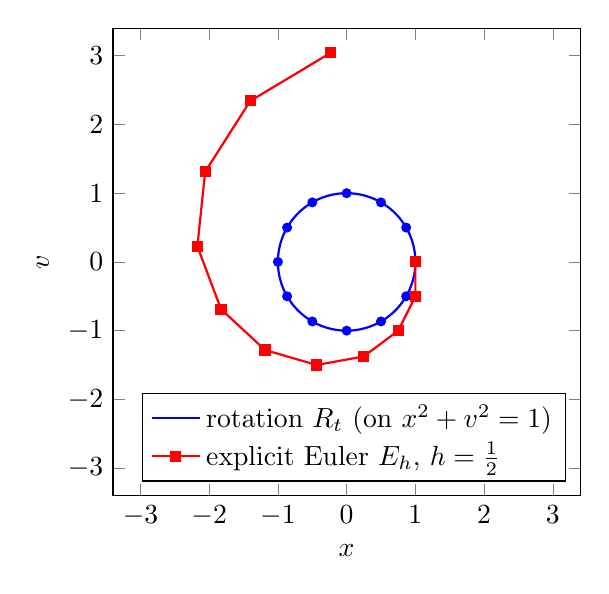
\begin{tikzpicture}
\begin{axis}[
    width=0.62\textwidth, height=0.62\textwidth,
    axis equal image,
    xlabel={$x$}, ylabel={$v$},
    xmin=-3.4, xmax=3.4, ymin=-3.4, ymax=3.4,
    xtick={-3,-2,-1,0,1,2,3},
    ytick={-3,-2,-1,0,1,2,3},
    legend pos=south east,
    legend cell align=left,
]
% exact orbit: unit circle
\addplot[blue, thick, domain=0:360, samples=181] ({cos(x)},{sin(x)});
\addlegendentry{rotation $R_t$ (on $x^2+v^2=1$)}
% rotation iterates, angle 30 degrees
\addplot[blue, only marks, mark=*, mark size=1.6pt, forget plot] coordinates {
(1,0) (0.8660,-0.5) (0.5,-0.8660) (0,-1) (-0.5,-0.8660)
(-0.8660,-0.5) (-1,0) (-0.8660,0.5) (-0.5,0.8660) (0,1)
(0.5,0.8660) (0.8660,0.5)
};
% explicit Euler iterates, h = 1/2, start (1,0)
\addplot[red, thick, mark=square*, mark size=1.6pt] coordinates {
(1,0) (1,-0.5) (0.75,-1) (0.25,-1.375) (-0.4375,-1.5)
(-1.1875,-1.28125) (-1.828125,-0.6875) (-2.171875,0.2265625)
(-2.05859375,1.3125) (-1.40234375,2.341796875)
(-0.2314453125,3.04296875)
};
\addlegendentry{explicit Euler $E_h$, $h=\tfrac12$}
\end{axis}
\end{tikzpicture}
\caption{Phase portrait of the harmonic oscillator.
Rotation iterates (dots, step angle $\pi/6$) remain on the unit circle
by \cref{eq:rotnorm}.
Explicit Euler iterates (squares, $h = \tfrac{1}{2}$, ten steps from
$(1,0)$) spiral outward: each step multiplies the squared norm by
$1 + h^2 = \tfrac{5}{4}$ by \cref{eq:eulernorm}, so the tenth iterate
has squared norm $(5/4)^{10} \approx 9.3$.}
\label{fig:phase}
\end{figure}

\subsection{Invariants and first integrals}

\begin{definition}[Invariant-preserving map, level structure]
\label{def:invariant}
Let $I : X \to \Real$.
A self-map $\Phi$ is \emph{invariant-preserving} for $I$ when
$I(\Phi\,x) = I\,x$ for all $x$
(machine-checked, \texttt{InvariantPreserving}).
For $c \in \Real$ the \emph{level structure} is
$P_{I = c} = \mathrm{crisp}_{\{x \,:\, I\,x = c\}}$.
On $X = \Real^2$ define the radial energy, the quarter-turn, and the
contraction:
\[
  H(x,y) = x^2 + y^2,
  \qquad
  \rho(x,y) = (-y,\, x),
  \qquad
  \sigma(x,y) = \Bigl(\tfrac{x}{2},\, \tfrac{y}{2}\Bigr).
\]
\end{definition}

\begin{theorem}[First-integral preservation]
\label{thm:firstintegral}
\begin{enumerate}[label=\textup{(\alph*)},nosep]
\item An invariant-preserving map for $I$ preserves $P_{I=c}$ for every
  $c$
  (machine-checked, \texttt{invariantPreserving\_preserves\_crisp}).
\item $\rho$ is invariant-preserving for $H$:
  $H(\rho(x,y)) = (-y)^2 + x^2 = H(x,y)$
  (machine-checked, \texttt{rot90\_firstIntegralPreserving}); hence it
  preserves every energy level set
  (machine-checked, \texttt{rot90\_preserves\_levelSets}).
\item $\sigma$ satisfies $H(\sigma\,p) = H(p)/4 < H(p)$ for every
  $p \neq (0,0)$
  (machine-checked, \texttt{shrink\_strictly\_dissipative}), so it is
  not invariant-preserving
  (machine-checked, \texttt{shrink\_not\_firstIntegralPreserving}),
  and its pointwise energy-conservation score is $0$ off the origin
  (machine-checked, \texttt{shrink\_energyScore\_zero}).
\end{enumerate}
\end{theorem}
\begin{proof}
(a) $I\,x = c$ and $I(\Phi\,x) = I\,x$ give $I(\Phi\,x) = c$.
(b) Direct computation, as displayed.
(c) $H(\sigma(x,y)) = \tfrac{x^2}{4} + \tfrac{y^2}{4} = H(x,y)/4$, and
$H(p) > 0$ for $p \neq (0,0)$, so $H(p)/4 < H(p)$.
\end{proof}

%=============================================================================
\section{Geometric and Conservative Integrators}
\label{sec:geometric}
%=============================================================================

The structures of this section are the ones geometric
integration~\cite{hairer2006}, conservative
discretization~\cite{leveque2002}, and compatible finite
elements~\cite{arnold2006} were built to keep.
We formalize their linear and toy cases and read each off the scale of
\cref{sec:scale}; the full nonlinear theories remain the cited
literature's.

\subsection{Symplectic $2 \times 2$ maps}

\begin{definition}[Symplectic structure]
\label{def:symplectic}
Let
\[
  J = \begin{pmatrix} 0 & 1 \\ -1 & 0 \end{pmatrix}.
\]
A matrix $A \in \Real^{2 \times 2}$ is \emph{symplectic} when
$A^{\top} J A = J$
(machine-checked, \texttt{Symplectic}); the associated structure is
$P_{\mathrm{sp}} = \mathrm{crisp}_{\{A \,:\, A^{\top} J A = J\}}$
(machine-checked, \texttt{symplecticScore},
\texttt{exactPreserves\_symplecticScore}).
\end{definition}

\begin{lemma}[Determinant identity]
\label{thm:detlemma}
For every $A \in \Real^{2 \times 2}$,
$A^{\top} J A = (\det A)\, J$
(machine-checked, \texttt{transpose\_mul\_J\_mul}).
\end{lemma}
\begin{proof}
Write $A = \begin{pmatrix} a & b \\ c & d \end{pmatrix}$.
Then
\[
  A^{\top} J
  = \begin{pmatrix} a & c \\ b & d \end{pmatrix}
    \begin{pmatrix} 0 & 1 \\ -1 & 0 \end{pmatrix}
  = \begin{pmatrix} -c & a \\ -d & b \end{pmatrix},
  \qquad
  A^{\top} J A
  = \begin{pmatrix} -c & a \\ -d & b \end{pmatrix}
    \begin{pmatrix} a & b \\ c & d \end{pmatrix}
  = \begin{pmatrix} 0 & ad - bc \\ -(ad - bc) & 0 \end{pmatrix},
\]
which is $(\det A)\,J$.
\end{proof}

\begin{theorem}[Determinant characterization]
\label{thm:sympdet}
$A^{\top} J A = J$ if and only if $\det A = 1$
(machine-checked, \texttt{symplectic\_iff\_det}).
\end{theorem}
\begin{proof}
By \cref{thm:detlemma}, $A^{\top} J A = J$ iff
$(\det A - 1)\,J = 0$.
Since $J \neq 0$ (its $(1,2)$ entry is $1$;
machine-checked, \texttt{J\_ne\_zero}), this holds iff
$\det A = 1$.
\end{proof}

\begin{proposition}[Symplectic and non-symplectic steps]
\label{thm:sympexamples}
\begin{enumerate}[label=\textup{(\alph*)},nosep]
\item The rotation
  $R_t = \begin{pmatrix} \cos t & -\sin t \\ \sin t & \cos t
  \end{pmatrix}$
  is symplectic for every $t$:
  $\det R_t = \cos^2 t + \sin^2 t = 1$
  (machine-checked, \texttt{symplectic\_rotation}).
\item The shear
  $\begin{pmatrix} 1 & s \\ 0 & 1 \end{pmatrix}$ is symplectic for
  every $s$: its determinant is $1$
  (machine-checked, \texttt{symplectic\_shear}).
\item The symplectic Euler step
  $\begin{pmatrix} 1 & h \\ -h & 1 - h^2 \end{pmatrix}$
  for $x' = v$, $v' = -x$ is symplectic:
  $\det = (1)(1 - h^2) - (h)(-h) = 1$
  (machine-checked, \texttt{symplecticEuler\_symplectic}).
\item The explicit Euler matrix
  $A_h = \begin{pmatrix} 1 & h \\ -h & 1 \end{pmatrix}$
  has $\det A_h = 1 + h^2$
  (machine-checked, \texttt{explicitEulerMatrix\_det}), so for every
  $h \neq 0$ it is not symplectic
  (machine-checked, \texttt{explicitEulerMatrix\_not\_symplectic});
  a non-unit scaling $\mathrm{diag}(2,2)$ fails with determinant $4$
  (machine-checked, \texttt{not\_symplectic\_scaling\_two}).
\end{enumerate}
\end{proposition}
\begin{proof}
Each determinant is a two-by-two computation;
Theorem~\ref{thm:sympdet} converts it to symplecticity.
\end{proof}

The matrix $A_h$ is the linear map $E_h$ of \cref{sec:circle}: its
determinant $1 + h^2$ and its norm growth factor \cref{eq:eulernorm}
are the same defect read through two structures, area and norm.
The spiral of \cref{fig:phase} is what $\det = 1 + h^2$ looks like in
phase space.

\subsection{Finite-volume mass conservation}

\begin{definition}[Mass structure, flux update]
\label{def:fv}
Fix $n \ge 1$ and work on the periodic grid
$X = \{u : \mathbb{Z}/n\mathbb{Z} \to \Real\}$.
The \emph{total mass} is $m(u) = \sum_{i} u_i$
(machine-checked, \texttt{totalMass}); the mass-$\mu$ structure is
$P_\mu = \mathrm{crisp}_{\{u \,:\, m(u) = \mu\}}$
(machine-checked, \texttt{massScore}).
Given face fluxes $F : \mathbb{Z}/n\mathbb{Z} \to \Real$ (with $F_i$
the flux through face $i - \tfrac{1}{2}$), the \emph{finite-volume
update} and the pointwise damping are
\[
  (\Phi_F\,u)_i = u_i - (F_{i+1} - F_i),
  \qquad
  (D_\lambda\,u)_i = (1 - \lambda)\,u_i .
\]
\end{definition}

\begin{theorem}[Telescoping mass conservation]
\label{thm:fv}
For every flux field $F$,
\begin{equation}
\label{eq:telescope}
  \sum_{i \in \mathbb{Z}/n\mathbb{Z}} \bigl(F_{i+1} - F_i\bigr) = 0,
\end{equation}
hence $m(\Phi_F\,u) = m(u)$ for every state $u$, and $\Phi_F$
preserves $P_\mu$ for every target mass $\mu$
(machine-checked, \texttt{flux\_telescope},
\texttt{fvUpdate\_conserves}, \texttt{fvUpdate\_preserves}).
The damping $D_{1/2}$ does not: on the single-cell grid with $u = (1)$,
the mass drops from $1$ to $\tfrac{1}{2}$
(machine-checked, \texttt{dampUpdate\_breaks\_mass},
\texttt{dampUpdate\_not\_preserves}).
\end{theorem}
\begin{proof}
The map $i \mapsto i + 1$ is a bijection of
$\mathbb{Z}/n\mathbb{Z}$, so
$\sum_i F_{i+1} = \sum_i F_i$ and \cref{eq:telescope} follows.
Then
$m(\Phi_F\,u) = \sum_i u_i - \sum_i (F_{i+1} - F_i) = m(u)$.
For the damping, $m(D_{1/2}\,u) = \tfrac{1}{2}\,m(u) \neq m(u)$ when
$m(u) = 1$.
\end{proof}

\begin{figure}[ht]
\centering
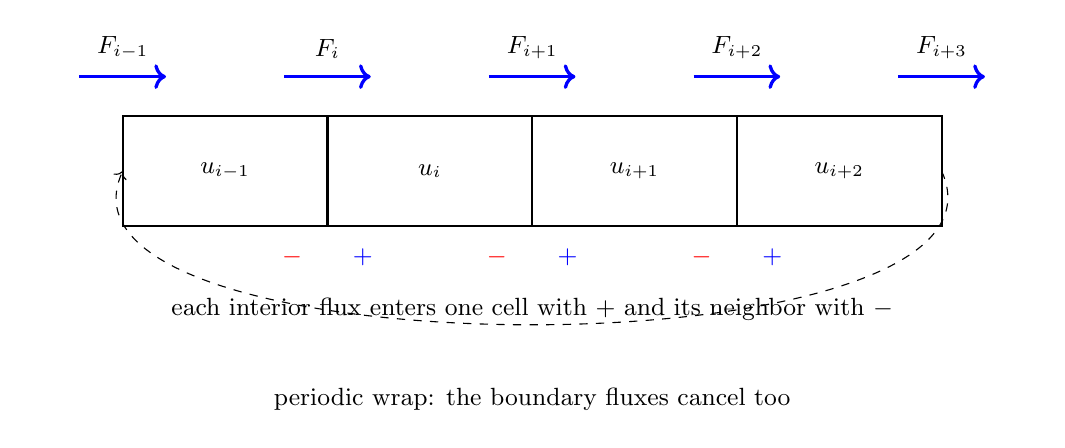
\begin{tikzpicture}[scale=1.0, every node/.style={font=\small}]
  % cells
  \foreach \i/\lab in {0/{u_{i-1}}, 1/{u_{i}}, 2/{u_{i+1}}, 3/{u_{i+2}}}
    {
      \draw[thick] (2.6*\i,0) rectangle (2.6*\i+2.6,1.4);
      \node at (2.6*\i+1.3,0.7) {$\lab$};
    }
  % face fluxes
  \foreach \i/\lab in {0/{F_{i-1}}, 1/{F_{i}}, 2/{F_{i+1}}, 3/{F_{i+2}}, 4/{F_{i+3}}}
    {
      \draw[->,very thick,blue] (2.6*\i-0.55,1.9) -- (2.6*\i+0.55,1.9);
      \node[above] at (2.6*\i,2.0) {$\lab$};
    }
  % +/- bookkeeping under interior faces
  \foreach \i in {1,2,3}
    {
      \node[red]  at (2.6*\i-0.45,-0.4) {$-$};
      \node[blue] at (2.6*\i+0.45,-0.4) {$+$};
    }
  \node at (5.2,-1.05)
    {each interior flux enters one cell with $+$ and its neighbor with $-$};
  % periodic wrap
  \draw[->,dashed] (10.4,0.7) .. controls (11.6,-1.9) and (-1.2,-1.9) .. (0,0.7);
  \node at (5.2,-2.2) {periodic wrap: the boundary fluxes cancel too};
\end{tikzpicture}
\caption{Telescoping fluxes on a periodic grid
(\cref{def:fv}).
Cell $i$ receives $F_i$ and loses $F_{i+1}$; summing over the cycle,
every flux appears once with each sign, so
$\sum_i (F_{i+1} - F_i) = 0$ \cref{eq:telescope} and the total mass is
conserved exactly (Theorem~\ref{thm:fv}).}
\label{fig:fv}
\end{figure}

\subsection{Positivity under a step-size bound}

\begin{definition}[Decay step]
\label{def:ssp}
For $c, \Delta t \ge 0$, one explicit Euler step of the linear decay
$u' = -c u$ is
\[
  S_{c,\Delta t}(u) = u - c\,\Delta t\,u = (1 - c\,\Delta t)\,u .
\]
The structure is $P_{\ge 0}$ of \cref{def:positivity}
(machine-checked, \texttt{uStep}, \texttt{positiveScore}).
\end{definition}

\begin{theorem}[Positivity iff the step-size bound]
\label{thm:ssp}
Let $c, \Delta t \ge 0$.
\begin{enumerate}[label=\textup{(\alph*)},nosep]
\item If $c\,\Delta t \le 1$, then $S_{c,\Delta t}$ preserves
  $P_{\ge 0}$: for $u \ge 0$,
  $S_{c,\Delta t}(u) = (1 - c\,\Delta t)\,u \ge 0$
  (machine-checked, \texttt{uStep\_nonneg},
  \texttt{uStep\_preserves\_score}).
\item If $c\,\Delta t > 1$, it does not: for $u > 0$,
  $S_{c,\Delta t}(u) = (1 - c\,\Delta t)\,u < 0$.
  Concretely, $c = \Delta t = u = 2$ gives $c\,\Delta t = 4 > 1$ and
  $S_{2,2}(2) = 2 - 8 = -6 < 0$
  (machine-checked, \texttt{uStep\_neg\_outside\_region},
  \texttt{uStep\_not\_preserves\_outside\_region}).
\end{enumerate}
Hence $S_{c,\Delta t}$ preserves positivity on all nonnegative states
if and only if $c\,\Delta t \le 1$.
\end{theorem}
\begin{proof}
Both parts read off the factored form: the step multiplies $u$ by
$1 - c\,\Delta t$, which is nonnegative exactly when
$c\,\Delta t \le 1$.
\end{proof}

The bound $c\,\Delta t \le 1$ is the strong-stability-preserving
(CFL-type) admissibility condition~\cite{gottlieb2001}: outside it the
status is inadmissible, not merely a larger error.

\subsection{Lie-group steps and constraint manifolds}

\begin{definition}[Group structure, paired schemes]
\label{def:liegroup}
On $X = \mathbb{C}$, let
$P_{G} = \mathrm{crisp}_{\{z \,:\, |z|^2 = 1\}}$, the unit circle as
the rotation group $SO(2)$
(machine-checked, \texttt{groupScore}).
For $g, w \in \mathbb{C}$ define the group step and the additive
coordinate step:
\[
  G_g(z) = g z, \qquad C_w(z) = z + w .
\]
\end{definition}

\begin{proposition}[Manifold preservation]
\label{thm:liegroup}
If $|g|^2 = 1$ then $G_g$ preserves $P_G$, since
$|g z|^2 = |g|^2 |z|^2 = |z|^2$
(machine-checked, \texttt{groupStep\_normSq},
\texttt{groupStep\_preserves}).
The coordinate step $C_{1/2}$ does not: $|1|^2 = 1$ but
$|1 + \tfrac{1}{2}|^2 = \tfrac{9}{4} \neq 1$
(machine-checked, \texttt{coordStep\_breaks\_group},
\texttt{coordStep\_not\_preserves}).
\end{proposition}

The coordinate error $|w| = \tfrac{1}{2}$ is small; the structural
verdict is still degree $0$.
This is the defining virtue of a Lie-group
integrator~\cite{iserles2000}: the update lives in the group.

\begin{definition}[Divergence-free structure]
\label{def:divfree}
On the periodic grid of \cref{def:fv}, the discrete divergence is
$(\delta u)_i = u_{i+1} - u_i$ and the constraint is
$\mathrm{DivFree}(u) :\iff \delta u = 0$
(machine-checked, \texttt{ddiv}, \texttt{DivFree});
the structure is
$P_{\delta = 0} = \mathrm{crisp}_{\mathrm{DivFree}}$
(machine-checked, \texttt{divFreeScore}).
\end{definition}

\begin{proposition}[Constraint preservation]
\label{thm:divfree}
The constant shift $u \mapsto u - c$ preserves $P_{\delta = 0}$, since
$(u_{i+1} - c) - (u_i - c) = u_{i+1} - u_i$
(machine-checked, \texttt{shift\_preserves}).
The single-coordinate bump (add $1$ at coordinate $0$) does not: on the
zero field over $\mathbb{Z}/3\mathbb{Z}$, the wrapped difference at
$i = 2$ becomes $1 \neq 0$
(machine-checked, \texttt{bump\_not\_preserves}).
A state off the constraint manifold scores $0$: it is structurally
inadmissible, not inaccurate
(machine-checked, \texttt{inadmissible\_off\_manifold}).
\end{proposition}

\subsection{Compatible discretization: $d_1 \circ d_0 = 0$}

\begin{definition}[Toy cochain complex]
\label{def:cochain}
On the periodic grid $\mathbb{Z}/(n{+}1)\mathbb{Z}$ define
\[
  (d_0 u)_i = u_{i+1} - u_i
  \quad (\text{node values} \to \text{edge values}),
  \qquad
  d_1 w = \sum_i w_i
  \quad (\text{edge values} \to \Real).
\]
An edge field $w$ is \emph{closed} when $d_1 w = 0$; the structure is
$P_{\ker d_1} = \mathrm{crisp}_{\{w \,:\, d_1 w = 0\}}$
(machine-checked, \texttt{compatibleScore}).
\end{definition}

\begin{theorem}[The cochain identity]
\label{thm:dd}
$d_1 \circ d_0 = 0$: for every node field $u$,
\[
  d_1(d_0 u) = \sum_i \bigl(u_{i+1} - u_i\bigr) = 0,
\]
so every discrete gradient is closed
(machine-checked, \texttt{closedGrad},
\texttt{d1\_comp\_d0\_eq\_zero}, \texttt{grad\_is\_compatible}).
The biased difference $(\tilde d_0 u)_i = u_{i+1} - 2 u_i$ breaks the
identity: on $u = (0, 1)$ over $\mathbb{Z}/2\mathbb{Z}$,
$d_1(\tilde d_0 u) = (1 - 0) + (0 - 2) = -1 \neq 0$
(machine-checked, \texttt{d0bad\_not\_compatible}).
\end{theorem}
\begin{proof}
The same reindexing bijection as in \cref{eq:telescope} cancels the
shifted sum against the unshifted one.
The biased scheme replaces $-u_i$ by $-2 u_i$, so the cancellation
fails by $\sum_i u_i$.
\end{proof}

A discretization is compatible when it reproduces the identity, the
discrete mirror of $d \circ d = 0$ in finite element exterior
calculus~\cite{arnold2006}; compatibility is a structural status, not
an accuracy order.

\subsection{Energy balance: three statuses on one scale}

\begin{definition}[Damped, forced scalar step]
\label{def:energy}
For state $x \in \Real$, energy $E(x) = x^2/2$, damping rate
$a \ge 0$, step $\Delta t$, and input $q$, define
\[
  \Phi_{a, \Delta t, q}(x) = x - a\,\Delta t\,x + \Delta t\,q
  = (1 - a\,\Delta t)\,x + \Delta t\,q .
\]
The pointwise structure is conservation,
$P_{E} = \mathrm{crisp}_{\{x \,:\, E(\Phi_{a,\Delta t,q}(x)) = E(x)\}}$
(machine-checked, \texttt{conserveScore}).
\end{definition}

\begin{theorem}[Exact balance law and its three regimes]
\label{thm:energy}
For all $a, \Delta t, q, x$,
\begin{equation}
\label{eq:balance}
  E\bigl(\Phi_{a,\Delta t,q}(x)\bigr)
  = E(x)
    - a\,\Delta t\Bigl(1 - \tfrac{a\,\Delta t}{2}\Bigr)x^2
    + \Delta t\,q\Bigl((1 - a\,\Delta t)\,x
      + \tfrac{\Delta t\,q}{2}\Bigr)
\end{equation}
(machine-checked, \texttt{energy\_balance\_law}).
Consequently:
\begin{enumerate}[label=\textup{(\alph*)},nosep]
\item \emph{conservation}: $a = 0$, $q = 0$ gives
  $E(\Phi(x)) = E(x)$ for all $x$, degree $1$ everywhere
  (machine-checked, \texttt{step\_conserves},
  \texttt{conserve\_degree\_one});
\item \emph{dissipation}: $q = 0$ and $0 \le a\,\Delta t \le 1$ give
  $E(\Phi(x)) \le E(x)$
  (machine-checked, \texttt{step\_dissipates}); at
  $a\,\Delta t = 1$, $x = 1$ the conservation score is $0$ while the
  zero threshold still holds
  (machine-checked, \texttt{dissipative\_threshold});
\item \emph{forcing}: $a = 0$, $\Delta t = q = 1$ is the translation
  $x \mapsto x + 1$, which conserves energy at $x = -\tfrac{1}{2}$
  (since $E(\tfrac{1}{2}) = E(-\tfrac{1}{2})$) and breaks it at
  $x = \tfrac{1}{2}$ (since $E(\tfrac{3}{2}) > E(\tfrac{1}{2})$):
  conservation is branch-dependent in the state
  (machine-checked, \texttt{forced\_branch\_dependent},
  \texttt{forced\_not\_preserves}).
\end{enumerate}
\end{theorem}
\begin{proof}
\Cref{eq:balance} is the expansion of
$\tfrac{1}{2}\bigl((1 - a\,\Delta t)x + \Delta t\,q\bigr)^2$:
the quadratic term is
$(1 - a\,\Delta t)^2 \tfrac{x^2}{2}
= \tfrac{x^2}{2} - a\,\Delta t(1 - \tfrac{a \Delta t}{2})x^2$,
the cross and source terms collect into the last summand.
(a) Set $a = q = 0$ in \cref{eq:balance}.
(b) With $q = 0$ the correction is
$-a\,\Delta t(1 - \tfrac{a\,\Delta t}{2})\,x^2 \le 0$ for
$0 \le a\,\Delta t \le 1$ (indeed for $a\,\Delta t \le 2$).
(c) Direct evaluation:
$E(\tfrac{1}{2}) = E(-\tfrac{1}{2}) = \tfrac{1}{8}$ but
$E(\tfrac{3}{2}) = \tfrac{9}{8} \neq \tfrac{1}{8}$.
\end{proof}

Conservation, dissipation, and forcing land at the three statuses
exact, threshold, and branch-dependent on one scale.

\subsection{Persistence as structural degree}

\begin{definition}[Persistence structure]
\label{def:persistence}
A feature born at $b$ and dying at $d$ ($b \le d$) has
\emph{persistence} $\mathrm{pers}(b,d) = d - b$.
At resolution $\varepsilon$ the structure is
$P_\varepsilon = \mathrm{crisp}_{\{d \,:\, \varepsilon \le d - b\}}$
(machine-checked, \texttt{persistence}, \texttt{statusScore}).
\end{definition}

\begin{proposition}[Persistence verdicts]
\label{thm:persistence}
\begin{enumerate}[label=\textup{(\alph*)},nosep]
\item The feature $(0,2)$ at resolution $1$ scores $1$
  (machine-checked, \texttt{long\_feature\_scores\_one});
  every zero-length feature $(b,b)$ at resolution $1$ scores $0$
  (machine-checked, \texttt{zero\_length\_feature\_scores\_zero}).
\item The score is monotone in the death time: $d \le d'$ and
  $P_\varepsilon(d) = 1$ imply $P_\varepsilon(d') = 1$
  (machine-checked, \texttt{statusScore\_mono\_death}); and antitone in
  the resolution: $\varepsilon' \le \varepsilon$ and
  $P_\varepsilon(d) = 1$ imply $P_{\varepsilon'}(d) = 1$
  (machine-checked, \texttt{statusScore\_mono\_eps}).
\end{enumerate}
\end{proposition}
\begin{proof}
(a) $1 \le 2 - 0$; $1 \le b - b = 0$ fails.
(b) $\varepsilon \le d - b \le d' - b$ and
$\varepsilon' \le \varepsilon \le d - b$.
\end{proof}

Long-lived features read as robust signal, short-lived ones as % slop-ok: stability term
filtration noise, matching the stability reading of persistence
diagrams~\cite{edelsbrunner2010}.

\subsection{Comparison on one scale}

Table~\ref{tab:comparison} reads the schemes of
\cref{sec:numerics,sec:geometric} off the single scale of
\cref{def:classes}.
Value order and structure degree are independent columns; a scheme can
score high on one and zero on the other.

\begin{table}[ht]
\centering
\small
\begin{tabular}{@{}lllll@{}}
\toprule
Scheme & Value error & Structure & Structure degree & Status \\
\midrule
Implicit update $\Phi_a$ & local $O(h^2)$ & nonnegativity & exact & checked \\
Explicit Euler $\Psi_h$ & local $O(h^2)$ & nonnegativity & $0$ for $x < h$ & checked \\
Mixing $\mathrm{mix}_a$ & exact mass & simplex & exact & checked \\
Scaling $\mathrm{scale}_2$ & n/a & simplex & $0$ (mass $2$) & checked \\
Midpoint $\Phi$ & exact at nodes & monotone pair & exact & checked \\
Averaging $A_{w,y}$ & local $O(w)$ & bound $[m,M]$ & exact & checked \\
Rotation $R_t$ & exact norm & unit circle & exact & checked \\
Explicit Euler $E_h$ & local $O(h^2)$ & unit circle & $0$ (norm ${\times}(1{+}h^2)$) & checked \\
Quarter-turn $\rho$ & exact energy & level set of $H$ & exact & checked \\
Contraction $\sigma$ & n/a & level set of $H$ & $0$ off origin & checked \\
Rotation, shear, sympl.\ Euler & exact & $A^{\top}JA = J$ & exact ($\det = 1$) & checked \\
Explicit Euler matrix $A_h$ & local $O(h^2)$ & $A^{\top}JA = J$ & $0$ ($\det = 1{+}h^2$) & checked \\
Flux update $\Phi_F$ & exact mass & total mass & exact & checked \\
Damping $D_\lambda$ & n/a & total mass & $0$ & checked \\
Decay step, $c\,\Delta t \le 1$ & local $O(\Delta t)$ & nonnegativity & exact & checked \\
Decay step, $c\,\Delta t > 1$ & local $O(\Delta t)$ & nonnegativity & $0$ & checked \\
Group step $G_g$ & exact & $|z|^2 = 1$ & exact & checked \\
Coordinate step $C_w$ & $O(|w|)$ & $|z|^2 = 1$ & $0$ & checked \\
Shift, gradient $d_0$ & exact & $\delta = 0$, $\ker d_1$ & exact & checked \\
Bump, biased $\tilde d_0$ & n/a & $\delta = 0$, $\ker d_1$ & $0$ & checked \\
Undamped, unforced step & exact & energy balance & exact & checked \\
Damped / forced step & n/a & energy balance & threshold / branch & checked \\
Persistence $(0,2)$ vs $(b,b)$ & n/a & $\varepsilon \le \mathrm{pers}$ & $1$ vs $0$ & checked \\
\midrule
Nonlinear symplectic, FEEC, SSP & method order & full structure & exact &
  established~\cite{hairer2006,marsden2001,arnold2006,gottlieb2001} \\
\bottomrule
\end{tabular}
\caption{Value accuracy against structural admissibility.
``Checked'' rows are Lean theorems of this paper
(Theorems~\ref{thm:positivity}--\ref{thm:persistence}).
The ``established'' row records the full nonlinear methods of the
literature, of which we formalize only the linear and toy cases.}
\label{tab:comparison}
\end{table}

%=============================================================================
\section{Graded Topology}
\label{sec:topology}
%=============================================================================

\subsection{Clopen is a consistent conjunction}

A set that is both closed and open sounds like a contradiction, the way
conditioning on impossible evidence sounds explosive.
Neither is.

\begin{theorem}[Clopen expansion]
\label{thm:clopen}
In every topological space, for every set $s$:
\[
  \mathrm{IsClosed}(s) \iff \mathrm{IsOpen}(s^{c}),
  \qquad
  \mathrm{IsClopen}(s) \iff
  \mathrm{IsOpen}(s) \wedge \mathrm{IsOpen}(s^{c}).
\]
(Machine-checked, \texttt{isClosed\_iff\_isOpen\_compl},
\texttt{isClopen\_iff\_isOpen\_and\_isOpen\_compl}.)
\end{theorem}
\begin{proof}
Closedness is defined as openness of the complement, not as failure of
openness; substituting this definition into the clopen conjunction
gives two positive openness claims about different sets.
No instance of $P \wedge \neg P$ occurs.
\end{proof}

\begin{proposition}[Clopen verdicts depend on the ambient topology]
\label{thm:clopenexamples}
\begin{enumerate}[label=\textup{(\alph*)},nosep]
\item On the connected real line, $\mathrm{IsClopen}(s)$ iff
  $s = \emptyset$ or $s = \Real$
  (machine-checked, \texttt{real\_isClopen\_iff\_trivial});
  $\Real$ itself satisfies both conjuncts, its complement $\emptyset$
  being open
  (machine-checked, \texttt{univ\_real\_isOpen\_and\_isOpen\_compl}).
\item The singleton $\{0\} \subseteq \Real$ is clopen in the discrete
  topology and not clopen in the standard topology, where it is not
  even open
  (machine-checked, \texttt{singleton\_not\_isOpen\_real},
  \texttt{singleton\_clopen\_discrete\_not\_standard}).
\end{enumerate}
\end{proposition}

Each non-clopen verdict fails one positive conjunct of
Theorem~\ref{thm:clopen}; none asserts a contradiction.
This is the topological mirror of the no-explosion stance of the
credence framework toward conditioning on the impossible: naive
language reads paradox where the formal predicates are jointly
satisfiable~\cite{priest1979,belnap1977}.

\subsection{Graded sets and crisp recovery}

A \emph{graded set} on a carrier $U$ is a membership function
$s : U \to [0,1]$; it is \emph{crisp} when $s$ takes only the values
$0$ and $1$.
Complement is $\negc$ pointwise and intersection is $\conjc$
pointwise.

\begin{definition}[Graded topology]
\label{def:credtopology}
A \emph{graded topology} on $U$ is a family of \emph{open} graded sets
containing $\emptyset$ and $U$, closed under binary intersection and
arbitrary predicate unions.
A set is \emph{closed} when its complement is open, \emph{clopen} when
both; a map is \emph{continuous} when preimages of opens are open
(machine-checked, \texttt{CredTopology}, with
\texttt{clopen\_univ}, \texttt{clopen\_emptyset},
\texttt{continuous\_id}, \texttt{continuous\_comp}).
\end{definition}

\begin{theorem}[Crisp recovery of classical topology]
\label{thm:crisp-topology}
A graded topology all of whose opens are crisp induces a topological
space on $U$ in which a set of points $P$ is open exactly when its
crisp embedding is graded-open; equivalently, for crisp $s$, $s$ is
graded-open iff its carrier $\{x : s(x) = 1\}$ is classically open
(machine-checked, \texttt{toTopologicalSpace},
\texttt{isOpen\_iff\_open}, \texttt{open\_crisp\_iff\_isOpen}).
\end{theorem}
\begin{proof}
Under the bijection between crisp graded sets and predicates, the
closure laws of \cref{def:credtopology} become the axioms of a
topological space: the empty and universal predicates are open,
binary intersections of opens are open, and unions over arbitrary
families are open.
The recovery statement is then definitional.
\end{proof}

The graded layer adds no classical topology; it recovers it exactly on
the crisp fragment.

\subsection{Openness and closedness degrees}

\begin{definition}[Degrees]
\label{def:degrees}
For $U$ nonempty and a graded set $s$, the \emph{openness degree} and
\emph{closedness degree} are
\[
  O(s) = \inf_{x \in U} s(x),
  \qquad
  C(s) = O(s^{c}) = \inf_{x \in U} \bigl(1 - s(x)\bigr)
\]
(machine-checked, \texttt{opennessDegree},
\texttt{closednessDegree}).
\end{definition}

\begin{proposition}[Degree calculus]
\label{thm:degrees}
For all graded sets $s, t$ on nonempty $U$:
\begin{enumerate}[label=\textup{(\alph*)},nosep]
\item $C(s) \le \negc O(s) = 1 - O(s)$
  (machine-checked, \texttt{closednessDegree\_le\_neg});
\item $O(U) = 1$, $C(U) = 0$, $O(\emptyset) = 0$,
  $C(\emptyset) = 1$
  (machine-checked, \texttt{univ\_openness\_one},
  \texttt{univ\_closedness\_zero},
  \texttt{emptyset\_openness\_zero},
  \texttt{emptyset\_closedness\_one});
\item $s \subseteq t$ implies $O(s) \le O(t)$ and $C(t) \le C(s)$
  (machine-checked, \texttt{openness\_monotone},
  \texttt{closedness\_antitone});
\item $O(s) \conjc O(t) \le O(s \cap t)$, where intersection is the
  pointwise product
  (machine-checked, \texttt{inter\_openness\_ge\_conj}).
\end{enumerate}
\end{proposition}
\begin{proof}
(a) For any $x_0$:
$C(s) \le 1 - s(x_0) \le 1 - O(s)$, since $O(s) \le s(x_0)$.
(b) Constant membership functions have constant infima.
(c) Pointwise $s(x) \le t(x)$ passes to infima; complements reverse it.
(d) For every $x$,
$O(s)\,O(t) \le s(x)\,t(x)$ (products of nonnegative lower bounds), so
$O(s)\,O(t)$ is a lower bound of $x \mapsto s(x)\,t(x)$.
\end{proof}

\begin{proposition}[Crisp dichotomy]
\label{thm:crisp-deg}
If $s$ is crisp, then $O(s) \in \{0, 1\}$; moreover $O(s) = 0$ iff some
point has membership $0$, and $O(s) = 1$ iff $s = U$
(machine-checked, \texttt{crisp\_openness\_zero\_or\_one},
\texttt{crisp\_openness\_zero\_iff},
\texttt{crisp\_openness\_one\_iff\_univ}).
\end{proposition}
\begin{proof}
If some $s(x) = 0$ the infimum is $0$; otherwise crispness forces
$s \equiv 1$ and the infimum is $1$.
\end{proof}

\subsection{Threshold cuts and threshold clopenness}

\begin{definition}[Threshold cut]
\label{def:cut}
The \emph{$t$-cut} of a graded set $s$ is the crisp set
\[
  s_{[t]} = \{x \in U : t \le s(x)\}
\]
(machine-checked, \texttt{cut}).
\end{definition}

\begin{theorem}[The cut family]
\label{thm:cuts}
For every graded set $s$:
\begin{enumerate}[label=\textup{(\alph*)},nosep]
\item the cuts are antitone: $t_1 \le t_2$ implies
  $s_{[t_2]} \subseteq s_{[t_1]}$
  (machine-checked, \texttt{cut\_antitone});
\item $s_{[0]} = U$ and $s_{[1]} = \{x : s(x) = 1\}$
  (machine-checked, \texttt{cut\_zero}, \texttt{cut\_one}).
\end{enumerate}
\end{theorem}
\begin{proof}
(a) $t_1 \le t_2 \le s(x)$.
(b) Every value clears $0$; clearing $1$ forces equality since
$s(x) \le 1$.
\end{proof}

\begin{proposition}[The tent neighborhood]
\label{thm:tent}
Let $\mu(x) = \max(0,\, 1 - |x|)$ on $\Real$.
For every threshold $0 < t \le 1$,
\[
  \mu_{[t]} = \bigl[-(1 - t),\; 1 - t\bigr];
\]
in particular $\mu_{[1/2]} = [-\tfrac{1}{2}, \tfrac{1}{2}]$, a closed
set in the standard topology
(machine-checked, \texttt{cut\_tent\_eq\_Icc},
\texttt{cut\_tent\_half}, \texttt{isClosed\_cut\_tent\_half}).
\end{proposition}
\begin{proof}
For $t > 0$, $t \le \max(0, 1 - |x|)$ forces $t \le 1 - |x|$, i.e.\
$|x| \le 1 - t$; conversely $|x| \le 1 - t$ gives
$1 - |x| \ge t$.
\end{proof}

\begin{figure}[ht]
\centering
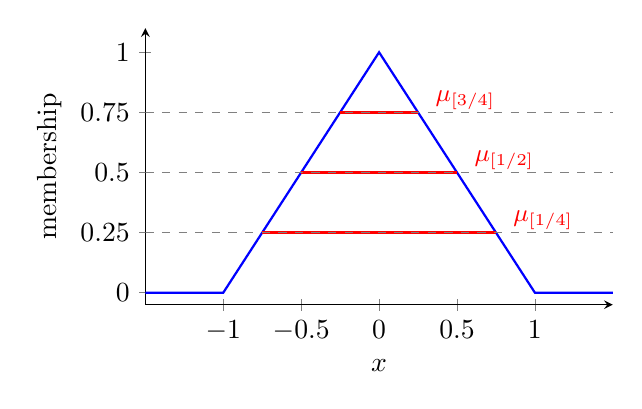
\begin{tikzpicture}
\begin{axis}[
    width=0.62\textwidth, height=0.42\textwidth,
    xlabel={$x$}, ylabel={membership},
    xmin=-1.5, xmax=1.5, ymin=-0.05, ymax=1.1,
    xtick={-1,-0.5,0,0.5,1},
    ytick={0,0.25,0.5,0.75,1},
    axis lines=left,
]
% tent profile
\addplot[blue, thick] coordinates {(-1.5,0) (-1,0) (0,1) (1,0) (1.5,0)};
% cuts as thick horizontal segments at their thresholds
\addplot[red,  very thick] coordinates {(-0.75,0.25) (0.75,0.25)};
\addplot[red,  very thick] coordinates {(-0.5,0.5)   (0.5,0.5)};
\addplot[red,  very thick] coordinates {(-0.25,0.75) (0.25,0.75)};
% threshold guides
\addplot[gray, dashed] coordinates {(-1.5,0.25) (1.5,0.25)};
\addplot[gray, dashed] coordinates {(-1.5,0.5)  (1.5,0.5)};
\addplot[gray, dashed] coordinates {(-1.5,0.75) (1.5,0.75)};
\node[red, anchor=west] at (axis cs:0.8,0.3)  {\small $\mu_{[1/4]}$};
\node[red, anchor=west] at (axis cs:0.55,0.55) {\small $\mu_{[1/2]}$};
\node[red, anchor=west] at (axis cs:0.3,0.8)  {\small $\mu_{[3/4]}$};
\end{axis}
\end{tikzpicture}
\caption{Nested threshold cuts of the tent profile
$\mu(x) = \max(0, 1 - |x|)$ (\cref{thm:tent}).
Each threshold $t$ cuts the graded neighborhood to the closed interval
$[-(1-t), 1-t]$; raising $t$ shrinks the cut
(Theorem~\ref{thm:cuts}(a)).}
\label{fig:tent}
\end{figure}

\begin{definition}[Threshold openness]
\label{def:topen}
Given degrees $O(s)$ and $C(s)$, the set $s$ is \emph{$t$-open} when
$t \le O(s)$, \emph{$t$-closed} when $t \le C(s)$, and
\emph{$t$-clopen} when both
(machine-checked, \texttt{IsOpenAt}, \texttt{IsClosedAt},
\texttt{IsClopenAt}).
\end{definition}

\begin{proposition}[Threshold-relative clopenness]
\label{thm:tclopen}
Clopen verdicts are antitone in the threshold: $t$-clopen implies
$t'$-clopen for every $t' \le t$
(machine-checked, \texttt{clopen\_antitone}).
They are not threshold-free: a set with $O(s) = 0.8$ and $C(s) = 0.7$
satisfies
\[
\begin{array}{c|ccc}
  t & \text{$t$-open} & \text{$t$-closed} & \text{$t$-clopen} \\
  \hline
  0.5 & \text{yes} & \text{yes} & \text{yes} \\
  0.75 & \text{yes} & \text{no} & \text{no} \\
  0.9 & \text{no} & \text{no} & \text{no}
\end{array}
\]
(machine-checked, \texttt{ex\_clopen\_at\_50},
\texttt{ex\_not\_clopen\_at\_75}, \texttt{ex\_not\_clopen\_at\_90}).
\end{proposition}
\begin{proof}
Antitonicity is transitivity of $\le$.
The table compares $0.5, 0.75, 0.9$ against $0.8$ and $0.7$.
\end{proof}

The cut threshold is the same designation parameter as in graded
consequence: threshold consequence is exactly inclusion of cuts of the
valuation-indexed graded sets of the premises into the conclusion's cut
(machine-checked, \texttt{thresholdConsequence\_iff\_cut}).

\subsection{Fuzzy open sets}

\begin{definition}[Fuzzy openness]
\label{def:fuzzyopen}
Over a topological space $U$, a graded set $s$ is \emph{fuzzy-open}
when its membership function is lower semicontinuous: for every $x$
and every $\alpha < s(x)$ there is a neighborhood of $x$ on which
$s > \alpha$
(machine-checked, \texttt{FuzzyOpen}; the empty and universal sets
qualify by \texttt{fuzzyOpen\_emptyset}, \texttt{fuzzyOpen\_univ}).
\end{definition}

\begin{theorem}[Fuzzy recovery]
\label{thm:fuzzy}
A crisp graded set $s$ is fuzzy-open iff its support
$\{x : s(x) = 1\}$ is classically open
(machine-checked, \texttt{crisp\_fuzzyOpen\_iff}).
\end{theorem}
\begin{proof}
Forward: take the witness $\alpha = 0$ at a support point; on the
resulting neighborhood $s > 0$, and crispness lifts this to $s = 1$,
so the support is a neighborhood of each of its points.
Backward: at a point with $\alpha < s(x)$, crispness gives
$s(x) = 1$, the support is an open neighborhood of $x$, and on it
$s = 1 > \alpha$.
\end{proof}

%=============================================================================
\section{The Crisp Fragment of Arithmetic and Analysis}
\label{sec:analysis}
%=============================================================================

\subsection{Laws at certainty}

Classical laws enter the scale at degree $1$ through
\cref{def:crisp}: a true decidable claim scores $1$, a false one $0$.

\begin{proposition}[Arithmetic at certainty]
\label{thm:arith}
With $\mathrm{eq}(a,b) = \mathrm{crisp}_{\{(a,b) \,:\, a = b\}}$ on
$\Nat^2$ and the analogous order and real scores:
\begin{enumerate}[label=\textup{(\alph*)},nosep]
\item $\mathrm{eq}(0 + n,\, n) = 1$ and $\mathrm{eq}(n + 0,\, n) = 1$
  for all $n \in \Nat$
  (machine-checked, \texttt{add\_zero\_left\_certain},
  \texttt{add\_zero\_right\_certain});
\item $n + 1 = m + 1$ implies $\mathrm{eq}(n, m) = 1$
  (machine-checked, \texttt{succ\_inj\_certain});
  the inequality $3 \le 7$ scores $1$
  (machine-checked, \texttt{three\_lt\_seven\_certain});
\item on $\Real$, the laws $a \le a$, $a + 0 = a$, $a \cdot 1 = a$, and
  $0 \le a^2$ all score $1$
  (machine-checked, \texttt{le\_refl\_certain},
  \texttt{add\_zero\_certain}, \texttt{mul\_one\_certain},
  \texttt{sq\_nonneg\_certain}).
\end{enumerate}
\end{proposition}
\begin{proof}
Each predicate holds classically; \cref{thm:endpoints}(e) converts the
proof into the score $1$.
\end{proof}

Not every real claim is certain: the score of $0 \le x$ is $1$ at
$x = 1$ and $0$ at $x = -1$, so the corresponding atom is
branch-dependent across the two evaluations, never interior
(machine-checked, \texttt{nonneg\_branchDependent}).

\subsection{Graded limits coincide with the standard limit}

\begin{definition}[Graded closeness, threshold limit]
\label{def:tlimit}
For $x, y \in \Real$ define the closeness credence
\[
  \mathrm{close}(x, y) = 1 - \min\bigl(|x - y|,\, 1\bigr) \in [0,1].
\]
For $t \in [0,1]$, the \emph{$t$-neighborhood} of $L$ is
$\{x : t \le \mathrm{close}(L, x)\}$, and a sequence $f$ has the
\emph{threshold limit} $L$ at $t$ when $f(n)$ lies in the
$t$-neighborhood of $L$ for all sufficiently large $n$
(machine-checked, \texttt{cClose}, \texttt{TNhd}, \texttt{TLimit}).
\end{definition}

\begin{lemma}[Closeness calculus]
\label{thm:cclose}
$\mathrm{close}(x,y) = 1$ iff $x = y$
(machine-checked, \texttt{cClose\_eq\_one\_iff});
$\mathrm{close}$ is symmetric
(machine-checked, \texttt{cClose\_comm});
and for $0 < t \le 1$,
\[
  t \le \mathrm{close}(x, y) \iff |x - y| \le 1 - t
\]
(machine-checked, \texttt{le\_cClose\_iff}).
\end{lemma}
\begin{proof}
$\mathrm{close}(x,y) = 1$ iff $\min(|x-y|, 1) = 0$ iff $|x-y| = 0$.
Symmetry is symmetry of $|x - y|$.
For the band: $t \le 1 - \min(|x-y|,1)$ iff
$\min(|x-y|,1) \le 1 - t$; since $t > 0$, $1 - t < 1$, the minimum is
attained by $|x-y|$, giving $|x-y| \le 1 - t$, and conversely.
\end{proof}

A single fixed threshold $t < 1$ is strictly coarser than the
classical limit: it only forces the tail into the band of radius
$1 - t$.
The classical limit is the meet over all thresholds.

\begin{theorem}[Graded limits are the standard limits]
\label{thm:tlimit}
For every sequence $f : \Nat \to \Real$ and $L \in \Real$:
\[
  \bigl(\forall\, t < 1:\; f \text{ has threshold limit } L
  \text{ at } t\bigr)
  \;\iff\;
  \lim_{n \to \infty} f(n) = L
\]
(machine-checked, \texttt{tlimit\_all\_iff\_tendsto}).
In particular the graded statement
$1/n \to 0$ holds at every threshold and equals the classical limit
(machine-checked, \texttt{tlimit\_one\_div},
\texttt{one\_div\_tlimit\_and\_classical}).
\end{theorem}
\begin{proof}
($\Rightarrow$)
Given $\varepsilon > 0$, set
$r = \min(\varepsilon/2,\, \tfrac{1}{2})$ and $t = 1 - r$; then
$0 < t < 1$.
The threshold limit at $t$ gives a tail with
$f(n)$ in the $t$-neighborhood of $L$, i.e.\
$|L - f(n)| \le 1 - t = r < \varepsilon$ by \cref{thm:cclose}.
($\Leftarrow$)
Given $t < 1$: for $t = 0$ the $t$-neighborhood is all of $\Real$ and
the condition is vacuous.
For $t > 0$, the radius $\rho = 1 - t$ is positive, so the classical
limit yields a tail with $|f(n) - L| < \rho$, which by
\cref{thm:cclose} places $f(n)$ in the $t$-neighborhood.
\end{proof}

The graded layer adds vocabulary, not a new analysis: a limit
statement is certain, an approximation at fixed tolerance is a
threshold statement, and the meet of the thresholds is exactly the
Mathlib limit.

\subsection{A robustness audit}
\label{sec:audit}

The last instantiation applies the status scale to mathematical claims
themselves.
A \emph{branch} assigns a credence to every atom; a family of branches
is the set of admissible assumption packages; a claim $\varphi$ is
evaluated in each branch.

\begin{definition}[Audit verdicts]
\label{def:audit}
Over a branch family $B$, a claim $\varphi$ is
\emph{robust} when its value is $1$ in every branch of a nonempty $B$; % slop-ok: defined term
\emph{branch-dependent} when its value is $1$ in some branch and $0$ in
another, never interior; and
\emph{inadmissible} when $B$ is empty
(machine-checked, \texttt{Robust}, \texttt{BranchDependent}, % slop-ok: Lean name
\texttt{Inadmissible}, with the characterizations
\texttt{robust\_certain\_every\_branch}, % slop-ok: Lean name
\texttt{robust\_of\_all\_one}, \texttt{inadmissible\_iff\_nil}). % slop-ok: Lean name
\end{definition}

\begin{theorem}[Audit trichotomy with witnesses]
\label{thm:audit}
\begin{enumerate}[label=\textup{(\alph*)},nosep]
\item \emph{Crisp logic is robust.} % slop-ok: defined term
  In a branch assigning only $0$ or $1$, excluded middle evaluates to
  \[
    c \disjc \negc c = c + (1 - c) - c(1 - c) = 1 - c(1 - c),
  \]
  which equals $1$ exactly when $c \in \{0, 1\}$; hence
$\varphi \disjc \negc\varphi$ is robust over every nonempty family of % slop-ok: defined term
  crisp branches
  (machine-checked, \texttt{excluded\_middle\_certain\_crisp},
\texttt{excluded\_middle\_robust}). % slop-ok: Lean name
\item \emph{A choice-style atom is branch-dependent.}
  An atom valued $1$ in an accepting branch and $0$ in a rejecting one
is branch-dependent, hence not robust % slop-ok: defined term
  (machine-checked, \texttt{choice\_audit\_branch\_dependent},
\texttt{choice\_not\_robust}). % slop-ok: Lean name
\item \emph{Inconsistent assumptions are inadmissible.}
  The empty family makes every claim inadmissible and supports no
  theorem
  (machine-checked, \texttt{inconsistent\_inadmissible},
\texttt{inadmissible\_not\_robust}). % slop-ok: Lean name
\item The three verdicts are pairwise exclusive
  (machine-checked, \texttt{audit\_verdicts\_exclusive}).
\end{enumerate}
\end{theorem}
\begin{proof}
(a) $1 - c(1-c) = 1$ iff $c(1-c) = 0$ iff $c \in \{0,1\}$; on crisp
branches every atom, hence every formula value $c$, makes the
disjunction certain.
(b), (c) Direct evaluation of the classifier on the two-branch and
empty families.
(d) The classifier returns a single verdict.
\end{proof}

The audit is the status scale applied to mathematics: a result certain
in every admissible branch is robust; one that turns on an extra posit % slop-ok: defined term
(a choice-style atom) is branch-dependent; contradictory assumptions
remove every branch rather than licensing explosion, the same design
as conditioning on zero evidence.

%=============================================================================
\section{Conclusion}
\label{sec:conclusion}
%=============================================================================

One scale, three instantiations.
The scale (\cref{sec:scale}) is a structure degree in $[0,1]$ with an
exact class, a threshold knob, a crisp embedding, a composition monoid
(Theorem~\ref{thm:monoid}), and a single deterministic scoring recipe
(Theorem~\ref{thm:score}).
On numerics it separates value accuracy from structural admissibility:
explicit Euler is order-accurate and still scores $0$ on positivity,
the circle, and the symplectic form, with $\det A_h = 1 + h^2$ and the
norm factor $1 + h^2$ as the same defect in two structures
(Theorems~\ref{thm:positivity}--\ref{thm:sympdet},
Table~\ref{tab:comparison}).
On topology it expands clopenness into the consistent conjunction
$\mathrm{Open}(s) \wedge \mathrm{Open}(s^c)$, recovers classical open
sets on the crisp fragment, and makes clopen verdicts
threshold-relative (Theorems~\ref{thm:clopen},
\ref{thm:crisp-topology}, \cref{thm:tclopen}).
On analysis it puts the defining laws at certainty and proves the
graded limit equal to the standard one (Theorem~\ref{thm:tlimit}),
with the robustness audit (Theorem~\ref{thm:audit}) sorting claims % slop-ok: formal audit term
into robust, branch-dependent, and inadmissible. % slop-ok: formal audit verdict

The boundary stays fixed: the preservation theory, the topology, and
the analysis are established mathematics, reused without modification;
the checked content is the status layer and its instantiations; the
positioning claim, that one scale should carry all three, is argued by
the uniformity of Table~\ref{tab:comparison} and the shared
no-explosion design.
A structural breach is a local low degree, not a global catastrophe:
the dissipative contraction scores $0$ off the origin while the
quarter-turn scores $1$ on the same carrier, and an empty branch
family removes support instead of proving everything.
Whether the layer scales beyond linear and toy cases to production
multiphysics solvers is open; the language and its machine-checked
foundation are what this paper supplies.

\section*{Acknowledgements}

Anthropic's Claude was used as an assistant for both the Lean
formalization and the manuscript preparation.

%=============================================================================
% Bibliography
%=============================================================================

\bibliographystyle{plain}
\bibliography{../cred}

%=============================================================================
% APPENDICES
%=============================================================================
\appendix

%=============================================================================
\section{Lean Formalization}
\label{app:lean}
%=============================================================================

The results of this paper are formalized in Lean~4 with Mathlib.
The status scale and the numerical examples are in
\texttt{Cred/Approx} (\texttt{Structure}, \texttt{Score},
\texttt{Positivity}, \texttt{Simplex}, \texttt{Monotonicity},
\texttt{MaxPrinciple}, \texttt{NormCircle}, \texttt{Invariant},
\texttt{FirstIntegral}, \texttt{Symplectic}, \texttt{FiniteVolume},
\texttt{SSP}, \texttt{LieGroup}, \texttt{DivFree},
\texttt{Compatible}, \texttt{EnergyBalance}, \texttt{Persistence});
the topology in \texttt{Cred/Topology} (\texttt{Basic},
\texttt{Clopen}, \texttt{Graded}, \texttt{Threshold},
\texttt{Fuzzy}); arithmetic, limits, and the audit in
\texttt{Cred/Math} (\texttt{Nat}, \texttt{Reals}, \texttt{Metric},
\texttt{Robustness}).

\textbf{Design choices.}
A credence is a real number carrying proofs of $0 \le c$ and
$c \le 1$.
A structure is a function into credences; the preservation classes of
\cref{def:classes} are definitions, not type classes, so every example
instantiates them literally.
Crisp structures go through a single $0/1$ lifting of decidable
predicates; decidability of real equalities and orders is supplied
classically.
The graded degrees of \cref{sec:topology} use conditionally complete
infima over nonempty carriers.
Classical content is never reformalized: connectedness of $\Real$,
$\mathrm{Tendsto}$, $\mathrm{IsOpen}$, and
$\mathrm{Set.Icc}$ are Mathlib's, and the bridges
(Theorems~\ref{thm:crisp-topology}, \ref{thm:fuzzy},
\ref{thm:tlimit}) state exact recoveries rather than analogues.

\textbf{Key definitions:}

\medskip
\noindent
\texttt{def StructureDegree (P : X $\to$ Credence) (x : X) : Credence := P x}

\medskip
\noindent
\texttt{def ExactPreserves (P) (x) : Prop := StructureDegree P x = 1}

\medskip
\noindent
\texttt{def PreservesAt (t) (P) (x) : Prop := t $\le$ StructureDegree P x}

\medskip
\noindent
\texttt{def Preserves (P) ($\Phi$) : Prop := $\forall$ x, ExactPreserves P x $\to$ ExactPreserves P ($\Phi$ x)}

\medskip
\noindent
\texttt{def scoreEps (eps r : $\Real$) : $\Real$ := max 0 (min 1 (1 - r / eps))}

\medskip
\textbf{Verification:} \texttt{cd lean \&\& lake build}.
Toolchain: Lean 4.16.0 with Mathlib 4.16.0; no \texttt{sorry}, no
custom axioms.

\end{document}
